% Project Background

IMSAR is a local company based out of Springville, UT, that specializes in making compact radar systems more affordable and accessible for use in small air vehicles. Since their conception in 2004, they have fulfilled multiple contracts with the Department of Defense and have developed radar systems with applications ranging from fighting fires to detecting enemy troop movements.
~\\~\\
One of the radar positioning systems (RPS) currently produced and sold by IMSAR is a computer-controlled tilt and pan positioner that maintains a communication link with radar units installed on air vehicles. The operational situation for these units is to be in a stationary position 2 to 20 miles away from the target in-flight vehicle. The current design employs a tilt and pan positioner that has become obsolete. The goal of this project is to replace the tilt and pan positioner, install an onboard computer, and to improve upon the current design. The current design requires that the data processing be done remotely on an external machine and has a barely passable user interface. Our final design will eliminate the need for external data processing. Challenges include integrating a new onboard control computer and proper handshaking between subsystems. The new RPS will be tested against IMSAR's drones flying in the vicinity. We will validate system functionality by tracking the drone with a camera mounted to the RPS. IMSAR will provide the positioning gimbal, and as such designing a positioner is not within the scope of our project.\\

{
\begin{figure}[H]
\begin{center}

\captionsetup{justification=centering,margin=2cm}
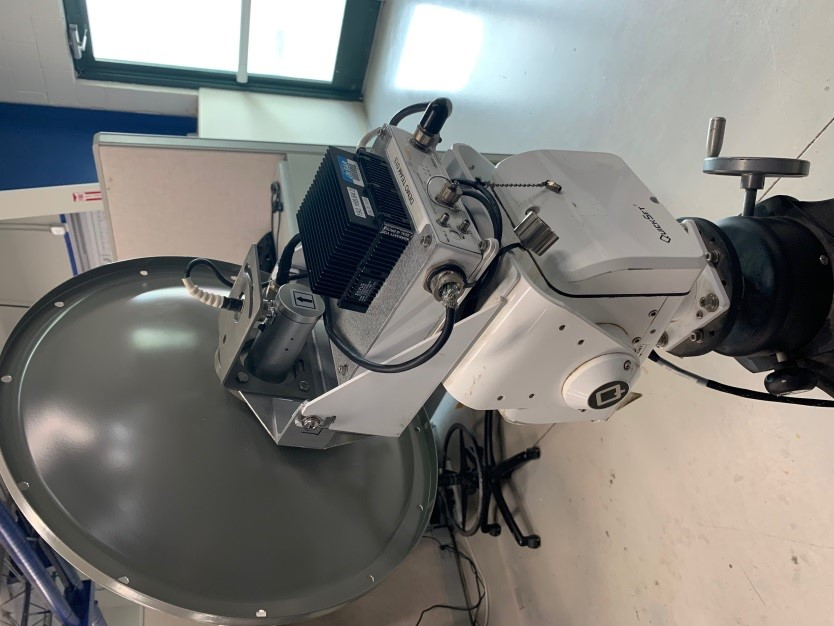
\includegraphics[angle=-90]{Images/IMSAR_PositioningSystem.jpg}
\caption{Current IMSAR Positioning System}
\end{center}
\end{figure}
}
